164. \begin{figure}[ht!]
\center{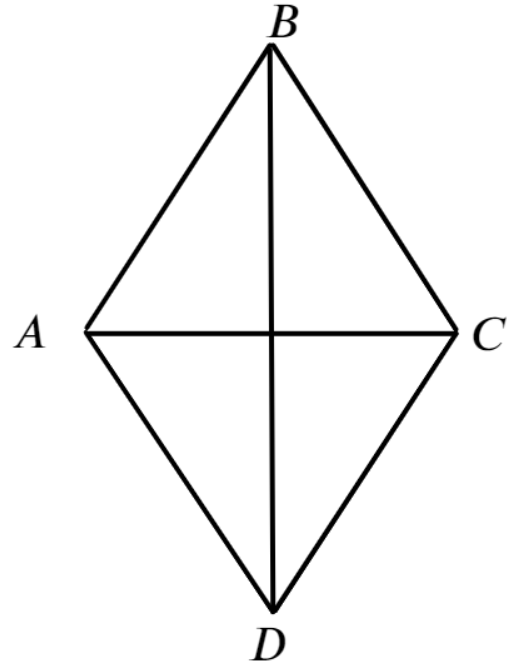
\includegraphics[scale=0.35]{g8-164.png}}
\end{figure}\\
Пусть стороны прямоугольника равны $a$см и $b$ см, тогда $\begin{cases}2(a+b)=100,\\ ab=616.\end{cases}\Leftrightarrow
\begin{cases}b=50-a,\\ a(50-a)=616.\end{cases}$\\$\Leftrightarrow
\begin{cases}b=50-a,\\ a^2-50a+616=0.\end{cases}\Leftrightarrow
\left[\begin{array}{l}\begin{cases}a=22\text{ см},\\ b=28\text{ см}.\end{cases}\\ \begin{cases}a=28\text{ см},\\ b=22\text{ см}.\end{cases}\end{array}\right.$
Значит, сторона ромба равна 22см. Тогда $S_{ABCD}=2S_{\Delta ABC}=2\cdot \cfrac{1}{2}\cdot 22\cdot22\cdot \sin(60^\circ)=242\sqrt{3}\text{ см}^2.$\\
